\chapter{Compensador Analogico} \chapterlabel{Informe/6-CompensadorAnalogico} \label{cap:Compensador Analogico}

\section{Compensador Analogico}

\noindent Se plantea una compensación como la que se muestra en la figura \ref{fig:diag-en-bloques-comp}. Está compuesta por un lazo de control interno con un controlador por adelanto de fase para lograr estabilizar el sistema, y un lazo de control externo con un integrador para eliminar el error en régimen permanente.

\begin{figure}[H]
	\centering
	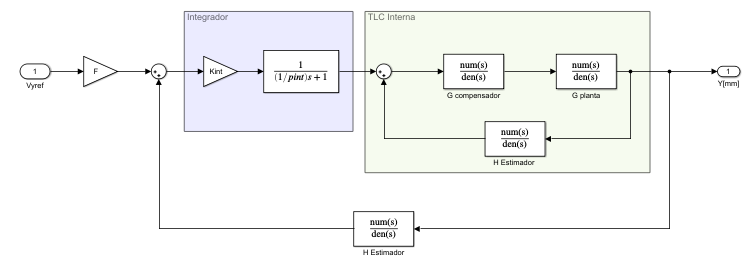
\includegraphics[scale=0.8]{Diagrama-en-bloques-comp.png}
	\caption{Diagrama del sistema completo.}
	\label{fig:diag-en-bloques-comp}
\end{figure}

\subsection{Diseño de compensador por adelanto de fase}

\noindent A partir de las transferencias de la planta, el controlador de corriente y el estimador de posición, se realizó el diseño de un compensador analógico por el método de adelanto de fase. Se llegó a la siguiente transferencia:


\begin{equation} 
	G_c(s) = 10*[20.346 * \frac{(s+44.3)}{(s+902.1)}]^2
\end{equation}

\noindent A continuación se diseña un circuito analógico correspondiente a este compensador.

\subsection{Diseño circuital}

\begin{figure}[H]
	\centering
	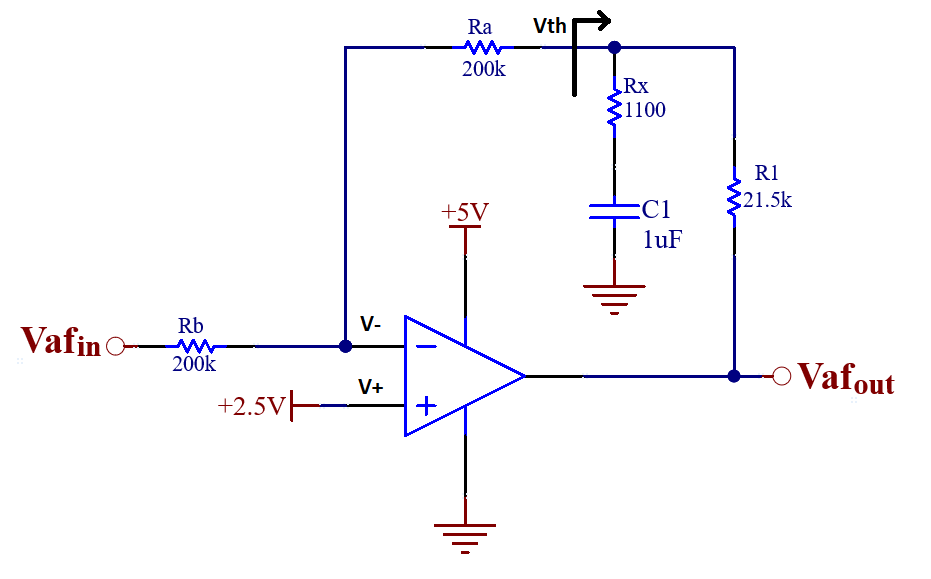
\includegraphics[scale=0.6]{Red-adelanto-fase.png}
	\caption{Diseño circuital de una red de adelanto de fase.}
	\label{fig:red-adelanto-fase}
\end{figure}


\noindent Para cada etapa del compensador por adelanto, se utilizará la topología mostrada en la figura \ref{fig:red-adelanto-fase}. Consiste en  un polo y cero con ganancia unitaria (si Ra = Rb). Luego se agrega la ganancia como una etapa separada.

\noindent La transferencia de lazo cerrado de esta etapa es:

\begin{equation} 
	\frac{V_{out}}{V_{in}}= - \frac{R_a}{R_b}*\frac{1+sC(R_x+R1)}{1+sCR_x}
\end{equation}

\noindent Por lo tanto, para tener polo = 902.1 Hz y zero = 44.3, y eligiendo el capacitor C = 1uF, resulta $R_x$ = 1100 y R1 = 21.5K. Además, se elige $R_a$ = $R_b$ = 200k para ganancia unitaria. Luego, la ganancia del compensador se obtiene con una etapa amplificadora.
Para ello, se utiliza un amplificador operacional como se muestra en la figura \ref{fig:ganancia-compensador}. Para lograr una ganancia de K=10 se utiliza $R_{322}$ = 1K y $R_{323}$ = 10K.


\begin{figure}[H]
	\centering
	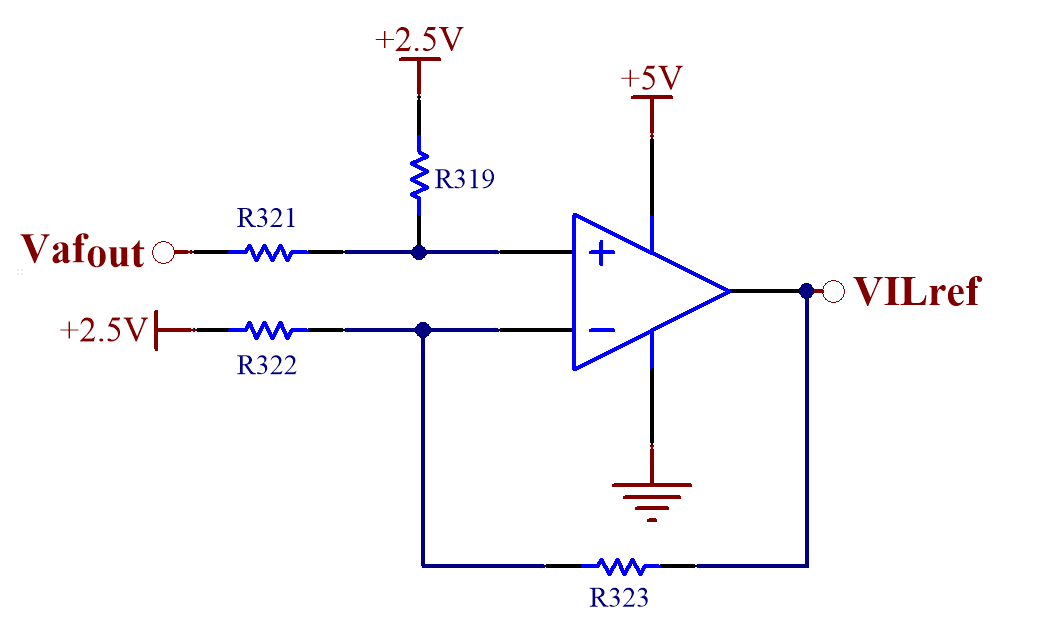
\includegraphics[scale=0.6]{Ganancia-compensador.png}
	\caption{Etapa de ganancia del compensador.}
	\label{fig:ganancia-compensador}
\end{figure}

\subsection{Compensador con integrador}

\noindent Para el análisis se tiene que la realimentación es:

\begin{equation} 
	H_{estim}=\frac{V_{estim}}{Y[m]}= - \frac{259.6}{(1 + \frac{s}{1Kr/s})*(1+\frac{s}{60Kr/s})^2}
\end{equation}

\noindent Y la cadena de avance, con m=30 Kg e Yo=5mm, es


\begin{equation} 
	G[m=30Kg] = TLC[m=30Kg] * G_{integrador}
\end{equation}

\noindent Podemos plantear un compensador del tipo:


\begin{equation} 
	G_{int} = K_{int} * \frac{1}{\frac{s}{P_{int}}+1}
\end{equation}

\noindent Por medio de la técnica de lugar de raíces y considerando P$_{int}$ =0.1 r/s se concluye que la ganancia del integrador que garantiza la estabilidad del sistema es $K_{int}$ = 50.

\subsubsection{Implementación circuital del integrador}

\noindent En la figura \ref{fig:circuito-integrador} se puede observar la topología y los valores utilizados en cada componente para el diseño del circuito integrador. 

\begin{figure}[H]
	\centering
	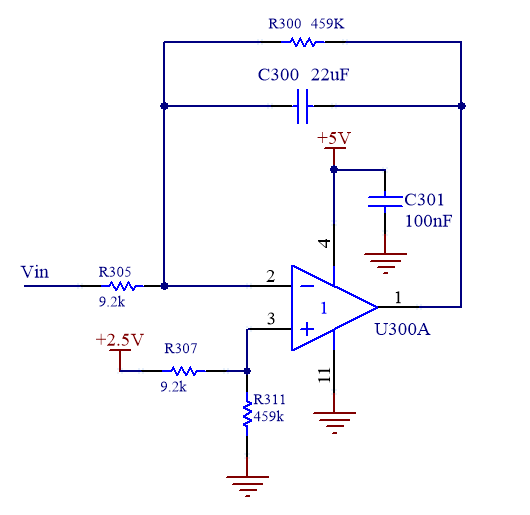
\includegraphics[scale=0.6]{Circuito-integrador.png}
	\caption{Implementación circuital del integrador.}
	\label{fig:circuito-integrador}
	\end{figure}

\subsubsection{Cálculo de ganancia de entrada}

\noindent Tomando la TLC' que corresponde a la ganancia total de los bloques con el integrador ya incorporado, la ganancia resulta:

\begin{equation} 
	Ganancia_{TLC'} \simeq \frac{1}{H_{estim}} = - \frac{1}{260}
\end{equation}

\begin{figure}[H]
	\centering
	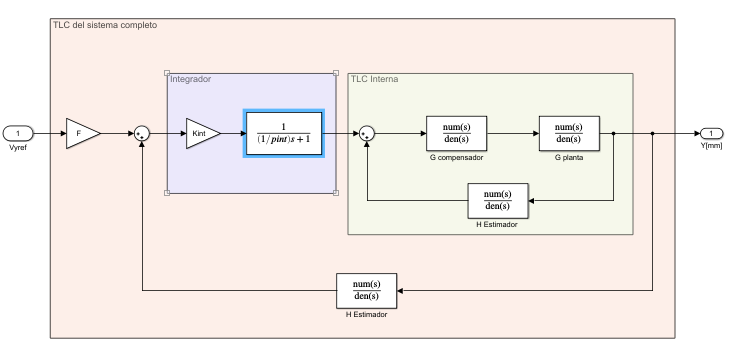
\includegraphics[scale=0.8]{Diagrama-en-bloques-compensador.png}
	\caption{Diagrama en bloques final.}
	\label{fig:diag-bloques-compensador}
\end{figure}

\noindent Por lo tanto teniendo tomando F=-1 y los rangos de posición de 1 mm a 5 mm como mínimo y máximo respectivamente se llega a lo siguiente:

\begin{equation} 
	Y[m] = F * (-\frac{1}{260})*V_{in} =\frac{1}{260}*V_{in} 
\end{equation}

\noindent La realimentación tiene un set-point de 3.4 V por lo tanto se le suma a Vin el mismo valor.

\noindent Los valores finales son:


\begin{table}[H]
	\begin{center}
		\begin{tabular}{| c | c |}
			\hline
			Y[mm] & $V_{in}[V]$\\ \hline
			5 & 4.7\\ \hline
			4 & 4.44 \\ \hline
			3 & 4.78\\ \hline
			2 &	3.92 \\ \hline		
		\end{tabular}
		\caption{Tensión de referencia $[V_{in}]$ Vs separación deseada [Y].}
		\label{tension-ref-vs-separacion-deseada}
	\end{center}
\end{table}

\subsubsection{Implementación circuital del bloque de ganancia de entrada “F”}

\noindent Para poder modificar la distancia de separación se ingresa al sistema con una tensión variable, la cual corresponde a una posición de referencia. Para ello se utiliza el circuito mostrado en la figura \ref{fig:etapa-de-entrada}.

\begin{figure}[H]
	\centering
	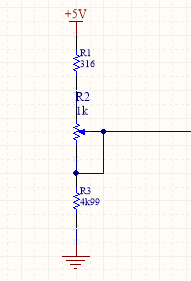
\includegraphics[scale=0.8]{Etapa-de-entrada.png}
	\caption{ Etapa de entrada.}
	\label{fig:etapa-de-entrada}
\end{figure}

 
 \noindent Se utiliza una resistencia variable de 1K y dos fijas. Para poder excursionar la tensión de referencia entre 3.92V y 4.7V, los valores de las resistencias R1 y R3 deben ser de 4911 y 313.5 respectivamente. 
 
\noindent Por lo tanto, adoptando un valor comercial para ellas, resulta:\\
\noindent R1 = 316 $\Omega$\\
\noindent R3 = 4990 $\Omega$
 
\noindent De esta forma, los valores de tensión para la referencia de posición quedan:\\
\noindent Tensión máxima= 4.69V\\
\noindent Tensión mínima = 3.96V
 
